\chapter{UML}
UML (\textbf{u}nified \textbf{m}odeling \textbf{l}anguage) è uno standard creato per unificare il modo di descrivere e progettare software in ambito della programmazione ad oggetti. 

\`E un linguaggio visuale che si basa su un meta-modello, un insieme di regole e vincoli per la modellazione di problemi software.
Ha una sintassi e una semantica ben definita. Uno dei vantaggi di UML è l'indipendenza dai linguaggi di programmazione.

I principali diagrammi trattati sono:
\begin{itemize}
\item diagrammi dei Casi d'Uso
\item diagrammi delle Classi
\item diagrammi dei Package
\item diagrammi di Sequenza
\item diagrammi di Attività
\end{itemize} 

\begin{figure}[H]
    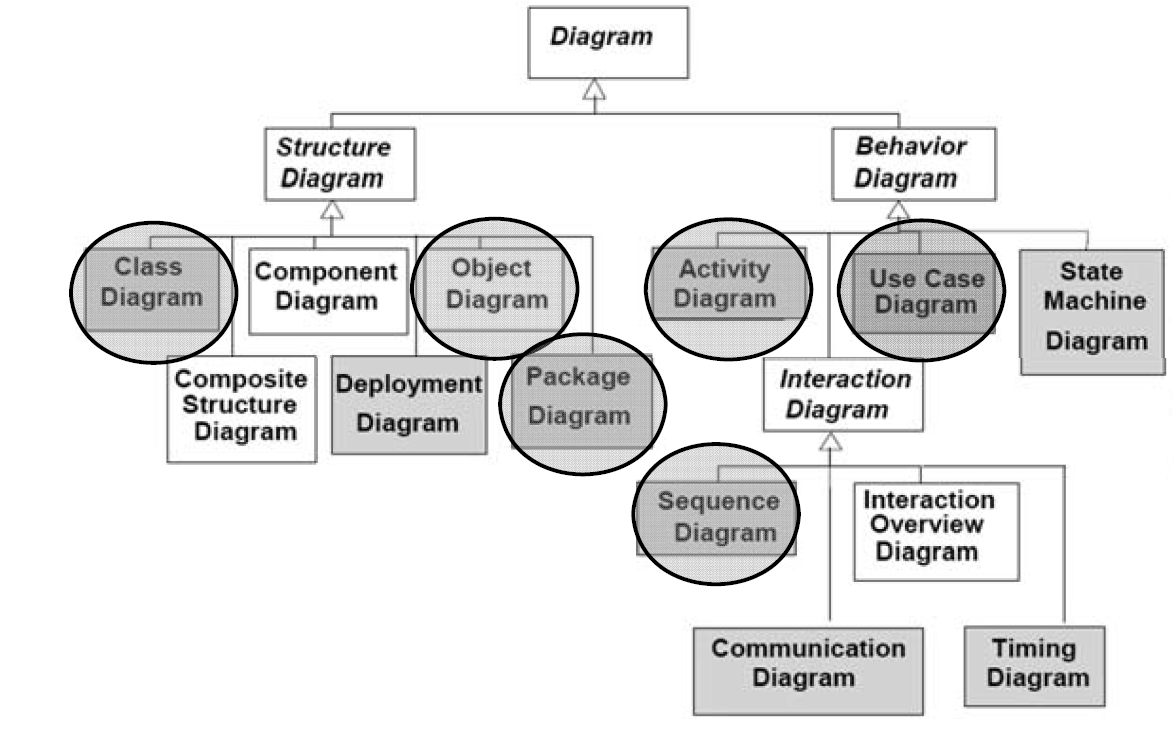
\includegraphics[width=1\textwidth]{res/img/diagrammiUML}
\end{figure}

\section{Diagrammi dei Casi d'Uso}

I diagrammi dei Casi d'Uso fanno parte dei diagrammi di comportamento. 

\subsection{I casi d'uso}
Un caso d'uso è un insieme di scenari (sequenze di azioni) che hanno in comune uno scopo finale (obiettivo) per un utente (attore),
\textit{cioè} un caso d'uso è una situazione nella quale il sistema viene utilizzato per soddisfare uno o più bisogno dell'utente.

Le funzionalità vengono descritte secondo la visione esterna, ovvero come vengono viste dall'utente, e non hanno nessun dettaglio implementativo.

I casi d'uso sono descrizioni puramente testuali, mentre i diagrammi dei casi d'uso vengono descritti con UML e rappresentano graficamente le relazioni tra attori e casi d'uso.

Un caso d'uso deve essere elementare, cioè non scomponibile in casi d'uso più semplici che abbiano ancora senso compiuto per gli attori coinvolti. Deve essere più grande di una singola operazione su un componente. 

Elementi di un caso d'uso:
\begin{itemize}
\item Nome + Identificatore - il nome deve essere più chiaro possibile;
\item Attori principali;
\item Attori secondari;
\item Pre-condizioni;
\item Post-condizioni; 
\item Scenario principale - la sequenza di azioni svolte dagli attori e dal sistema;
\item Scenari alternativi - eccezioni/errori e come devono essere gestiti;
\item Trigger - evento scatenante del caso d'uso.
\end{itemize}

\subsubsection{Attori}

Un attore è colui che svolge il caso d'uso per raggiungere un certo obiettivo. Può essere una persona o un altro sistema. 

Un utente può avere più ruoli (diversi attori); più utenti possono avere il medesimo ruolo (singolo attore). 

Un attore può essere collegato a più casi d'uso e un caso d'uso può avere più attori. \\
Come identificare un attore:
\begin{enumerate}
\item Identificare un entità
\item L'entità è una persona che interagisce con il sistema?
\begin{itemize}
\item[\texttt{SI}] $\to$ potrebbe essere un attore, ma si deve fare attenzione alle persone che potrebbero comunque essere parte del sistema.
\item[\texttt{NO}] $\to$ l'entità è qualcosa che si può cambiare all'interno del design del sistema?
\begin{itemize}
\item[\texttt{NO}] $\to$ probabilmente è un attore.
\item[\texttt{SI}] $\to$ l'entità non dovrebbe essere un attore, in quanto tutto ciò su cui è possibile avere il controllo, è da considerarsi parte del sistema.
\end{itemize}
\end{itemize}
\end{enumerate}

\subsection{I diagrammi}

I diagrammi dei casi d'uso sono grafi con gli attori e i casi d'uso come nodi, mentre gli archi rappresentano la comunicazione attore-caso d'uso e le relazioni tra casi d'uso, che possono essere:
\begin{itemize}
\item inclusione
\item estensione
\item generalizzazione
\end{itemize}

\begin{figure}[H]
    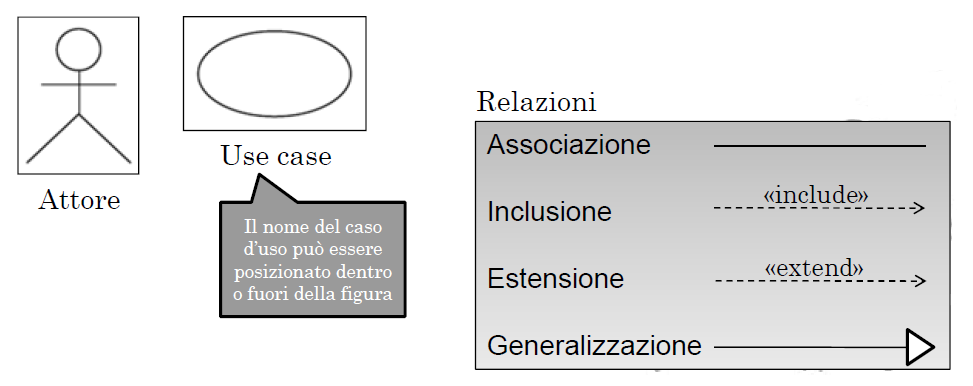
\includegraphics[width=1\textwidth]{res/img/componentiUseCaseDiagram}
    \caption{Componenti diagrammi dei Casi d'Uso (\textit{Slide E02})}
\end{figure}

\subsubsection{Inclusione}
L'inclusione viene utilizzata quando una funzionalità è comune a più casi d'uso. 
\texttt{A <<include>> B} indica che ogni istanza di A esegue B in modo incondizionato. 
A non conosce i dettagli di B, ma solo i risultati. Allo stesso modo, B non sa di essere incluso in A.

\subsubsection{Estensione}
L'estensione aumenta le funzionalità di un caso d'uso. 
\texttt{A <<extend>> B} indica che ogni istanza di A esegue B in modo condizionato, cioè l'esecuzione di B interrompe A.
Questa relazione viene spesso utilizzata per isolare in uno caso d'uso a parte la specifica di attività opzionali 
o eccezionali che potrebbero aver luogo durante l'esecuzione della funzione principale.

\subsubsection{Inclusione vs Estensione}
Entrambe le relazioni aumentano il comportamento di un caso d'uso e possono essere comuni a più casi d'uso. 
Nell'inclusione, un attore esegue sempre tutte le inclusioni, mentre nell'estensione l'attore può non esesguirle tutte.
Quindi, un'inclusione viene usata se una funzionalità si ripete in più casi d'uso; 
l'esetensione se si vogliono descrivere variazioni dalla funzionalità standard. 

\subsubsection{Generalizzazione}
La generalizzazione aggiunge o modifica delle caratteristiche di base. 
Può essere usato tra attori o tra casi d'uso (più raro). 
A è generalizzazione di B se B condivide almeno le funzionalità di A.

\subsection{Individuazione Casi d'Uso}

Definizione del contesto:
\begin{enumerate}
\item Identificazione attori e responsabilità
\item Identificazione degli obiettivi da raggiungere per ciascun attore (Primi approssimazione use case)
\item Valutare attori e use case e raffinarli (Divisione e accorpamento)
\item Trovare le relazioni di inclusione
\item Trovare le relazioni di estensione
\item Trovare le relazioni di generalizzazione
\end{enumerate}

Livello di dettaglio:
\begin{itemize}
\item Kite level - Livello molto astratto, definisce macro funzionalità
\item Sea level - Livello intermedio, utile nella scoperta di funzionalità nascoste
\item Fish level - Livello di dettaglio, da esso si individuano direttamente i requisiti del sistema
\end{itemize}

\section{Diagrammi delle Classi}
\section{Diagrammi dei Package}
\section{Diagrammi di Sequenza}
\section{Diagrammi di Attività}